\chapter{Introduction}


Actually the video devices capture a lot amount of information of some real world scene for processing in computing systems. With increasing of information, is necessary  to develop compression techniques for representing the video information with the lowest possible amount of bits for facilitating the storing and transmission. This advancements also have increased the requirements for video format as 4k(3840 $\times$ 2160px) and 8k(7680 $\times$ 4320px) for resolution, 10 bit depth and 50-60 for frame rate. Moreover, the advancement of technologies in the cloud for storing and computation, has prompted the use of services that use videos as streaming, video conference, IPTV among others, which has generated a significant increase in traffic of video over networks, in special for mobile applications, as can be seen in Fig. \ref{fig:vni}.

\begin{figure}[!h]
\centering
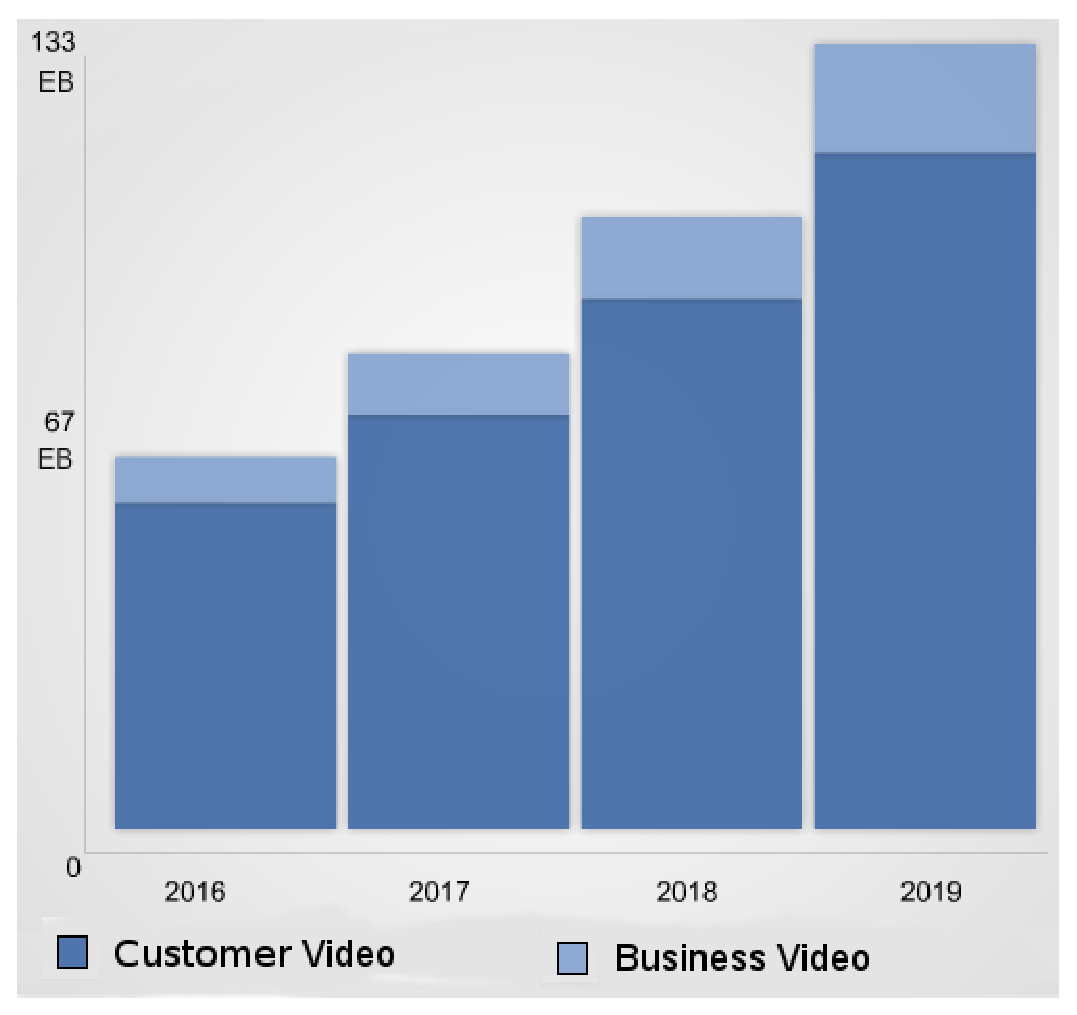
\includegraphics[width=0.4\textwidth]{images/vni.eps}
\caption[Estimated future global IP traffic growth for Video]{Estimated future global IP traffic growth for Video \scriptsize{Source: Cisco VNI Forecast}} 
\label{fig:vni}
\end{figure}

Video compression standards as MPEG4, H.264, VP9, HEVC among others have an important role in the transferring of video information through the cloud, looking with each generation of video encoders, increasingly reduce the bit rate. Conventional video encoders exploiting the correlation spatial and temporal between neighbour video frames. Instead of conventional video encoders, Compressive Sensing has emerged as a approach for simplifying the signal representation taking advantage of the sparse property of video signal which means that most of the signal coefficients are zero. Compressive sensing using a small number of sample for reconstruct a signal resolving a $\ell_p$- norm minimization problem using a trained dictionary of samples.\\

The main aim of video coding is to improve the coding efficiency, reducing the bit-rate for representing a video preserving a high level of quality with a maximum delay and complexity permitted. The complexity and bit-rate has been a important condition for video coding mainly in mobile applications due to processing and bandwidth limitations in the devices. Although cloud computing is a alternative for processing in devices with poor-resources, the latency is high. Fog Computing arise as a alternative, inside of cloud computing, for reducing the latency using the edge of the network for processing. \\


This project presents a proposal for video coding through the fog network using compressive sensing to reduce the bit-rate. Dictionary learning process and sparse representation of the signal are performed in the fog network and directed toward the cloud. Dictionary and sparse vector are transferred for reconstruct the video  in the end-user side.

\section{Problem Statement}

Nowadays, the video services in the cloud have increased significantly thanks to popularity of applications in video-on-demand, broadcasting, live streaming, internet and mobile network video, video chat, telepresence systems and video conferencing. The evolution of this services create a stronger needs in terms of transmission bandwidth and processing for video, specially for High Definition (HD) content as 1080p, and the emerged beyond-HD content as 4k and with 8k. This video content required a greater amount of bits for represent it with a quality level acceptable. As an example, Table \ref{fig:youtube} shows the bit rates necessary for representing a live stream video of Youtube with a specific resolution using H.264 encoder. 

\begin{table}[!h]
\centering
\begin{tabular}{|c|c|c|}
\hline
\textbf{Resolution} & \textbf{Min bit rate (Kbps)} & \textbf{Max bit rate (Kbps)} \\
\hline
2560$\times$1440$@$60 & 9000 & 18000 \\
\hline
2560$\times$1440$@$30 &  6000 & 13000  \\
\hline
1920$\times$1080$@$60 & 4500 & 9000\\
\hline
1920$\times$1080 & 3000 & 6000 \\
\hline
\end{tabular}
\caption[Bit rates requirements for some resolutions in Live Stream Video of Youtube]{Bit rates requirements for some resolutions in Live Stream Video of Youtube \scriptsize{Source: \url{https://support.google.com/youtube/answer/2853702}}}
\label{fig:youtube}
\end{table}

In addition to high bit rates requirements, in some regions there are limitations on  network bandwidth, for example, Latin America has a internet connectivity speed of 7,26 Mbps on average while for mobile networks has a lower speed to 4 Mbps on average \cite{cepal}. High bit rates and network bandwidth limitation involve continuous efforts to maximise the coding efficiency, reducing the bit rates considering aspects as data loss and the computational resources in this process. Another feature to consider in video cloud applications that require high use of bandwidth is the delay between the cloud provider and end devices. The distance and shared nature of the cloud makes the data transmission susceptible to multiple kinds of delay which affect the user experience. Also the increase tendency of devices connected to internet with Internet of Things (IoT) makes the problem even more relevant. \\


Conventional Video encoders, as VP9, MPEG4 and H.26x, exploits the spatial and temporal redundancy, also applying an entropy coding and quantization process to improve the coding efficiency. This encoders have been  widely deployed and the three main process have been widely development, for this reason in necessary seek and adapt to the convectional video encoders other strategies for encoding process that can maximise the compression capability. 


\section{Objectives}
\subsection{General Objective}
Reduce the bit rates
\subsection{Specific Objectives}
\begin{itemize}
\item
\item
\item
\item
\end{itemize}

\section{Project Scope}


